\PassOptionsToPackage{table}{xcolor}

\documentclass[aspectratio=169]{beamer}

\usetheme{auriga}
\usecolortheme{auriga}
\setbeamersize{text margin left=2em,text margin right=2em}

\usepackage{fontspec}
\usepackage{xcolor}
\usepackage{enumitem}
\usepackage{makecell}
\usepackage{tabularx}

% for vertical centering text in X column
\renewcommand\tabularxcolumn[1]{m{#1}}
\newcolumntype{C}{>{\centering\arraybackslash}X}

\setmainfont{PT Astra Serif}

\title{
  \huge{VXLAN} \\
  \vskip0pt plus 1filll
  \large{Что это, зачем нужен и почему не VLAN?}
}
\author{Швалов Даниил К33211}
\institute{Университет ИТМО}
\date{2023}

\begin{document}

% change itemize default label
\def\labelitemi{---}

\frame{\titlepage}

\begin{frame}
  \frametitle{Введение}

  \begin{figure}[H]
    \centering
    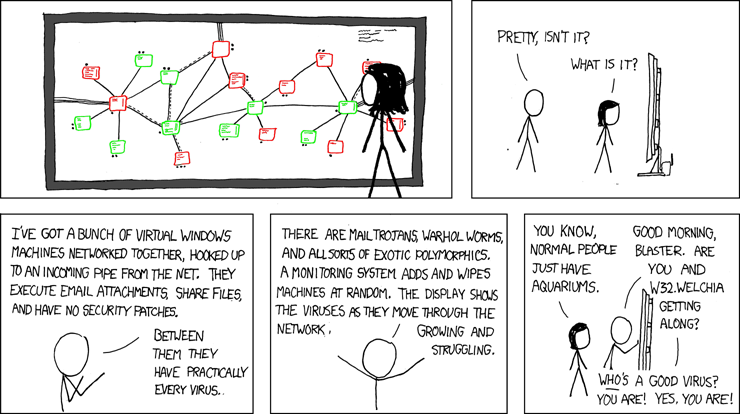
\includegraphics[width=0.5\textwidth]{images/xkcd.png}
  \end{figure}

  Представим, что мы являемся небольшим провайдером виртуальных машин. Пару дней
  назад крупный клиент захотел, чтобы машины могли общаться между собой по
  внутренней сети. Причем все это должно быть безопасно.

  \vspace*{1em}

  Первое, что приходит в голову --- это \textbf{VLAN}.
\end{frame}

\begin{frame}
  \frametitle{Что такое VLAN?}

  \begin{figure}[H]
    \centering
    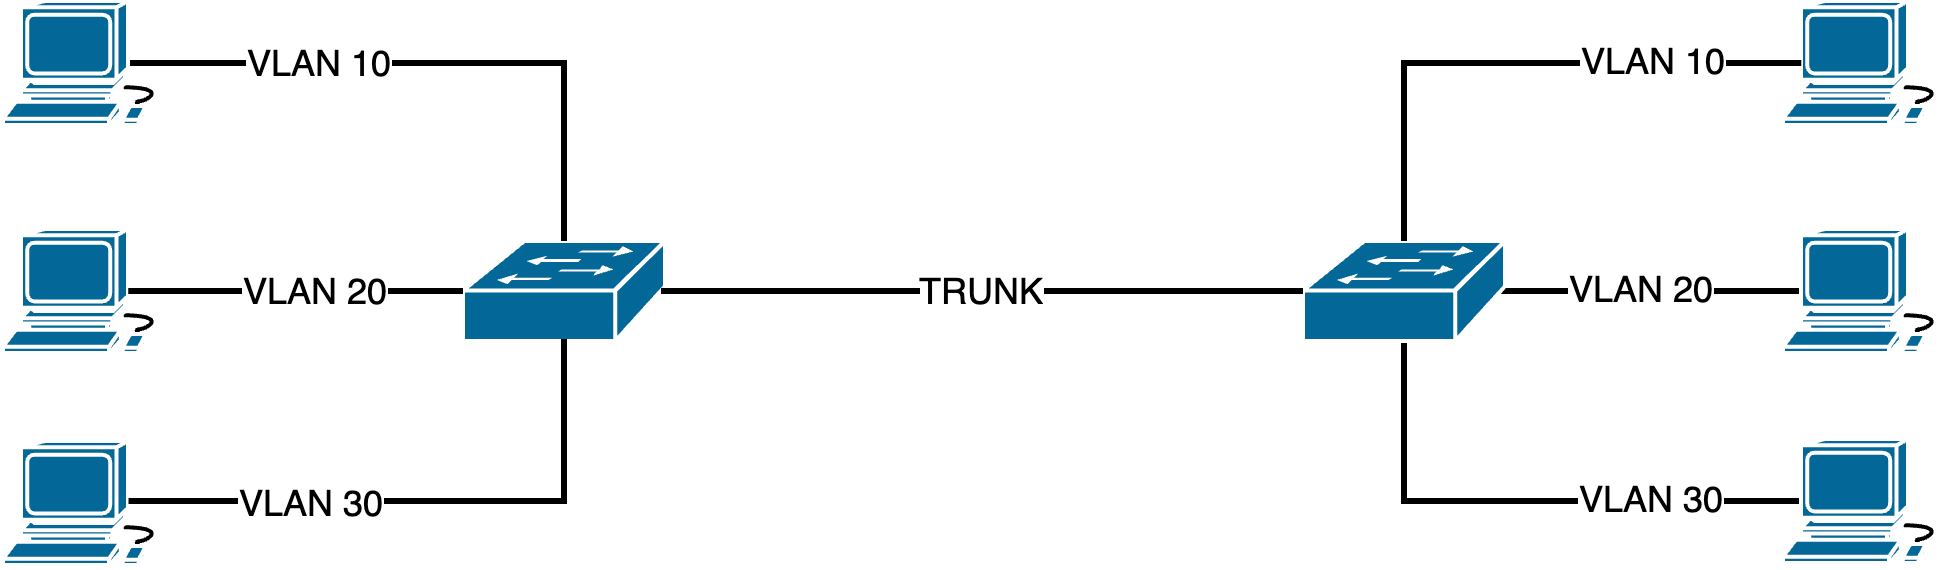
\includegraphics[width=0.8\textwidth]{images/vlan.png}
  \end{figure}

  \vspace*{1em}

  VLAN (Virtual Local Area Network) --- это технология, которая позволяет
  создавать группы устройств, имеющих возможность взаимодействовать между собой
  напрямую на канальном уровне, хотя физически при этом они могут быть подключены
  к разным коммутаторам.
\end{frame}

\begin{frame}
  \frametitle{Зачем нужен VLAN?}

  \begin{minipage}{0.45\textwidth}
    VLAN используется для:
    \vspace*{1em}
    \begin{itemize}
      \item гибкого разделения устройств на группы;
      \item уменьшения количества широковещательного трафика в сети;
      \item повышения безопасности и управляемости сети.
    \end{itemize}
  \end{minipage}
  \hspace*{1em}
  \begin{minipage}{0.45\textwidth}
    \centering
    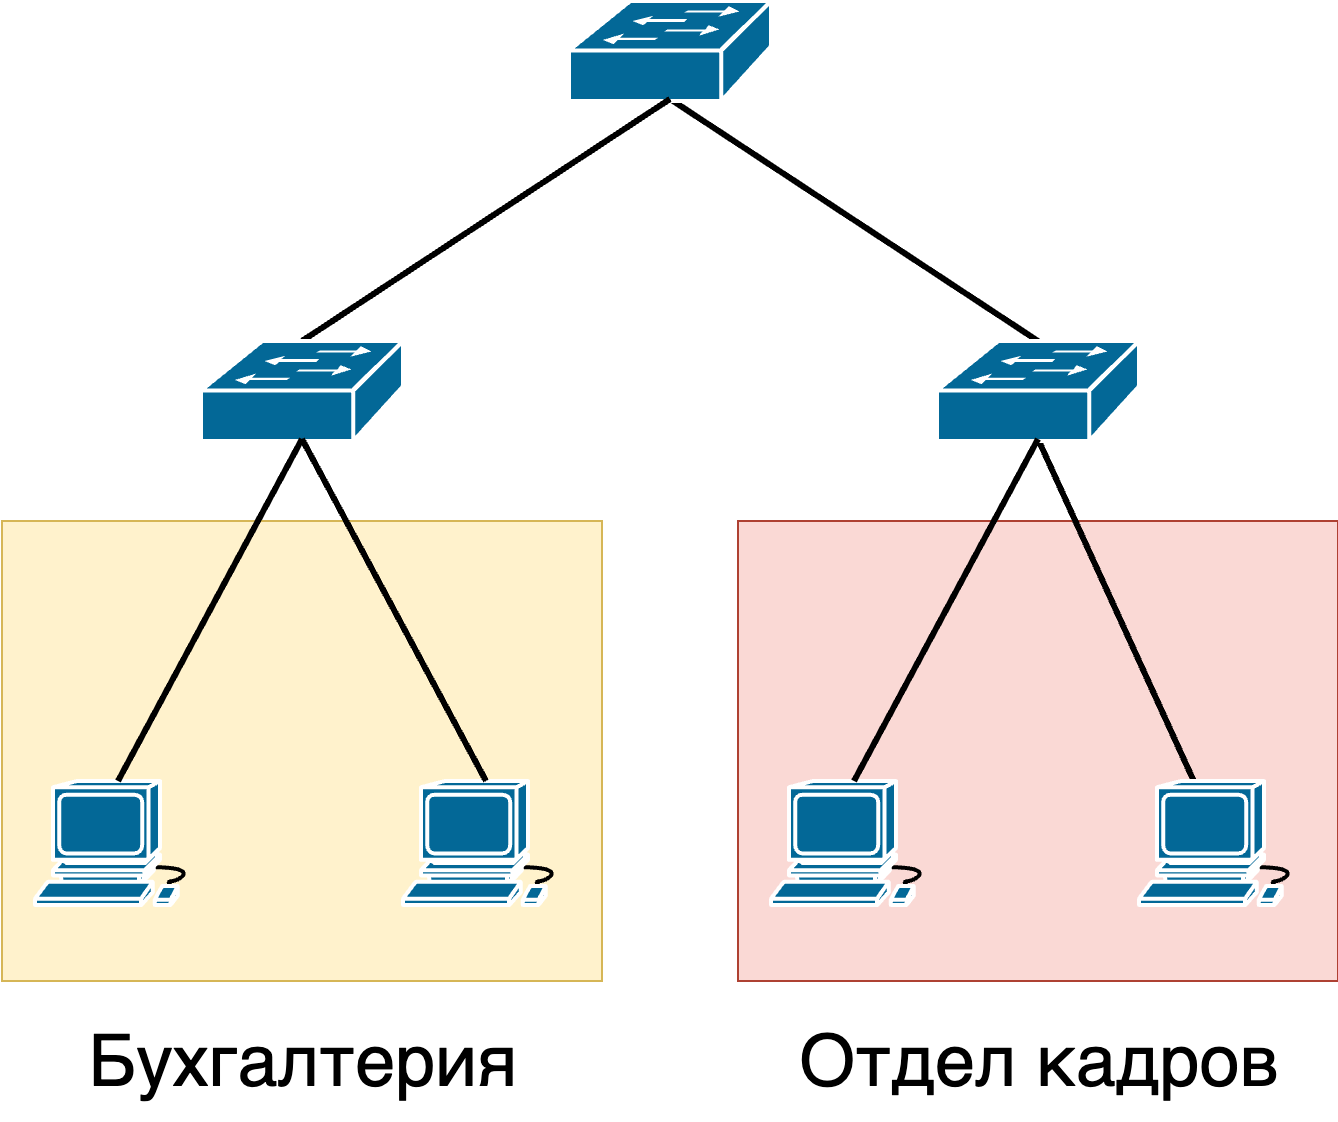
\includegraphics[width=0.9\textwidth]{images/vlan-example.png}
  \end{minipage}
\end{frame}

\begin{frame}
  \frametitle{Устройство VLAN}

  \begin{figure}[H]
    \centering
    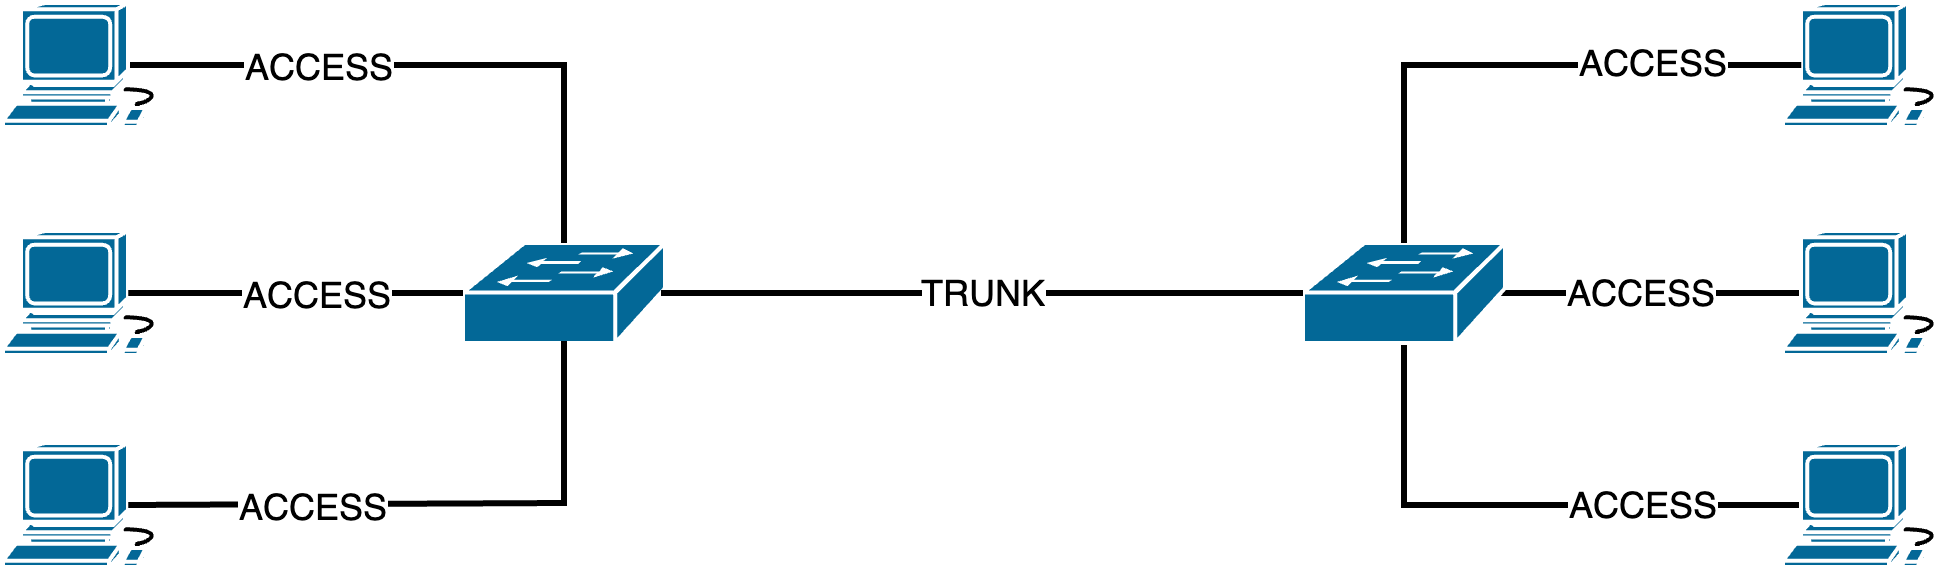
\includegraphics[width=0.8\textwidth]{images/vlan-access-trunk.png}
  \end{figure}

  \footnotesize

  \begin{itemize}[label=,leftmargin=0pt]
    \item \textbf{Access порт} --- это порт принадлежащий одному VLAN-у и
    передающий нетегированный трафик. Access порт может принадлежать только одному
    VLAN-у, по умолчанию это первый (нетегированный) VLAN. Любой кадр, который
    проходит через access порт, помечается номером, принадлежащим этому VLAN-у.
    \item \textbf{Trunk порт} --- это порт передающий тегированный трафик одного или нескольких
    VLAN-ов. Этот порт, наоборот, не изменяет тег, а лишь пропускает кадры с тегами,
    которые разрешены на этом порту.
  \end{itemize}

\end{frame}

\begin{frame}
  \frametitle{Формат кадра VLAN}

  Стандартный Ethernet кадр:
  \begin{center}
    \footnotesize
    \renewcommand*{\arraystretch}{3.0}
    \begin{tabularx}{\textwidth}{|c|c|c|C|c|}
      \hline
      \shortstack{Source MAC      \\ 6 байт}          &
      \shortstack{Destination MAC \\ 6 байт} &
      \shortstack{Type            \\ 2 байта}       &
      \shortstack{Payload         \\ 1500 байт} &
      \shortstack{FSC             \\ 4 байта}         \\
      \hline
    \end{tabularx}
  \end{center}

  \vspace*{1em}

  VLAN Ethernet кадр:
  \begin{center}
    \footnotesize
    \renewcommand*{\arraystretch}{3.0}
    \begin{tabularx}{\textwidth}{|c|c|c|c|C|c|}
      \hline
      \shortstack{Source MAC      \\ 6 байт}          &
      \shortstack{Destination MAC \\ 6 байт} &
      \shortstack{802.1Q Tag      \\ 4 байта} &
      \shortstack{Type            \\ 2 байта}       &
      \shortstack{Payload         \\ 1500 байт} &
      \shortstack{FSC             \\ 4 байта}         \\
      \hline
    \end{tabularx}
  \end{center}
\end{frame}

\begin{frame}
  \frametitle{Формат кадра VLAN}

  VLAN Ethernet кадр:
  \begin{center}
    \footnotesize
    \renewcommand*{\arraystretch}{3.0}
    \begin{tabularx}{\textwidth}{|c|c|c|c|C|c|}
      \hline
      \shortstack{Source MAC                      \\ 6 байт}          &
      \shortstack{Destination MAC                 \\ 6 байт} &
      \cellcolor{yellow!25}\shortstack{802.1Q Tag \\ 4 байта} &
      \shortstack{Type                            \\ 2 байта}       &
      \shortstack{Payload                         \\ 1500 байт} &
      \shortstack{FSC                             \\ 4 байта}         \\
      \hline
    \end{tabularx}
  \end{center}

  \vspace*{1em}

  Формат 802.1Q Tag:
  \begin{center}
    \footnotesize
    \renewcommand*{\arraystretch}{3.0}
    \begin{tabularx}{\textwidth}{|C|C|C|C|}
      \hline
      \shortstack{TPID \\ 16 бит}          &
      \shortstack{PCP  \\ 3 бита} &
      \shortstack{DEI  \\ 1 бит} &
      \shortstack{VID  \\ 12 бит} \\
      \hline
    \end{tabularx}
  \end{center}

  \vspace*{1em}

  \begin{itemize}[label=,leftmargin=0pt]
    \item \textbf{Tag Protocol Identifier}: указывает какой протокол
    используется для тегирования.
    \item \textbf{Priority code point}: используется для задания приоритета
    передаваемого трафика.
    \item \textbf{Drop eligible indicator}: используется для указания кадров,
    которые могут быть отброшены в случае перегрузки.
    \item \textbf{VLAN Identifier}: указывает какому VLAN принадлежит кадр.
  \end{itemize}
\end{frame}

\begin{frame}
  \frametitle{Самое время задаться вопросом}

  \begin{center}
    \LARGE{Отлично, все работает. \\ Но зачем тогда нужен VXLAN?}
  \end{center}
\end{frame}

\begin{frame}
  \frametitle{Недостатки VLAN}

  1. Количество подсетей не может быть больше, чем 4094 (0 или 4095
  зарезервированы), поскольку VID всего 12 бит.
  \begin{center}
    \footnotesize
    \renewcommand*{\arraystretch}{3.0}
    \begin{tabularx}{\textwidth}{|C|C|C|C|}
      \hline
      \shortstack{TPID                     \\ 16 бит}          &
      \shortstack{PCP                      \\ 3 бита} &
      \shortstack{DEI                      \\ 1 бит} &
      \cellcolor{yellow!25}\shortstack{VID \\ 12 бит} \\
      \hline
    \end{tabularx}
  \end{center}

  Этого недостаточно для больших облачных провайдеров.

  \vspace*{2em}

  2. VLAN работает на втором уровне модели OSI. Это вносит свои ограничения, в
  частности, VLAN не подходит для межсетевого туннелирования.
\end{frame}

\begin{frame}
  \frametitle{А это значит, что}

  \begin{center}
    \LARGE{VXLAN спешит на помощь!}
  \end{center}
\end{frame}

\begin{frame}
  \frametitle{VXLAN}

  \begin{figure}[H]
    \centering
    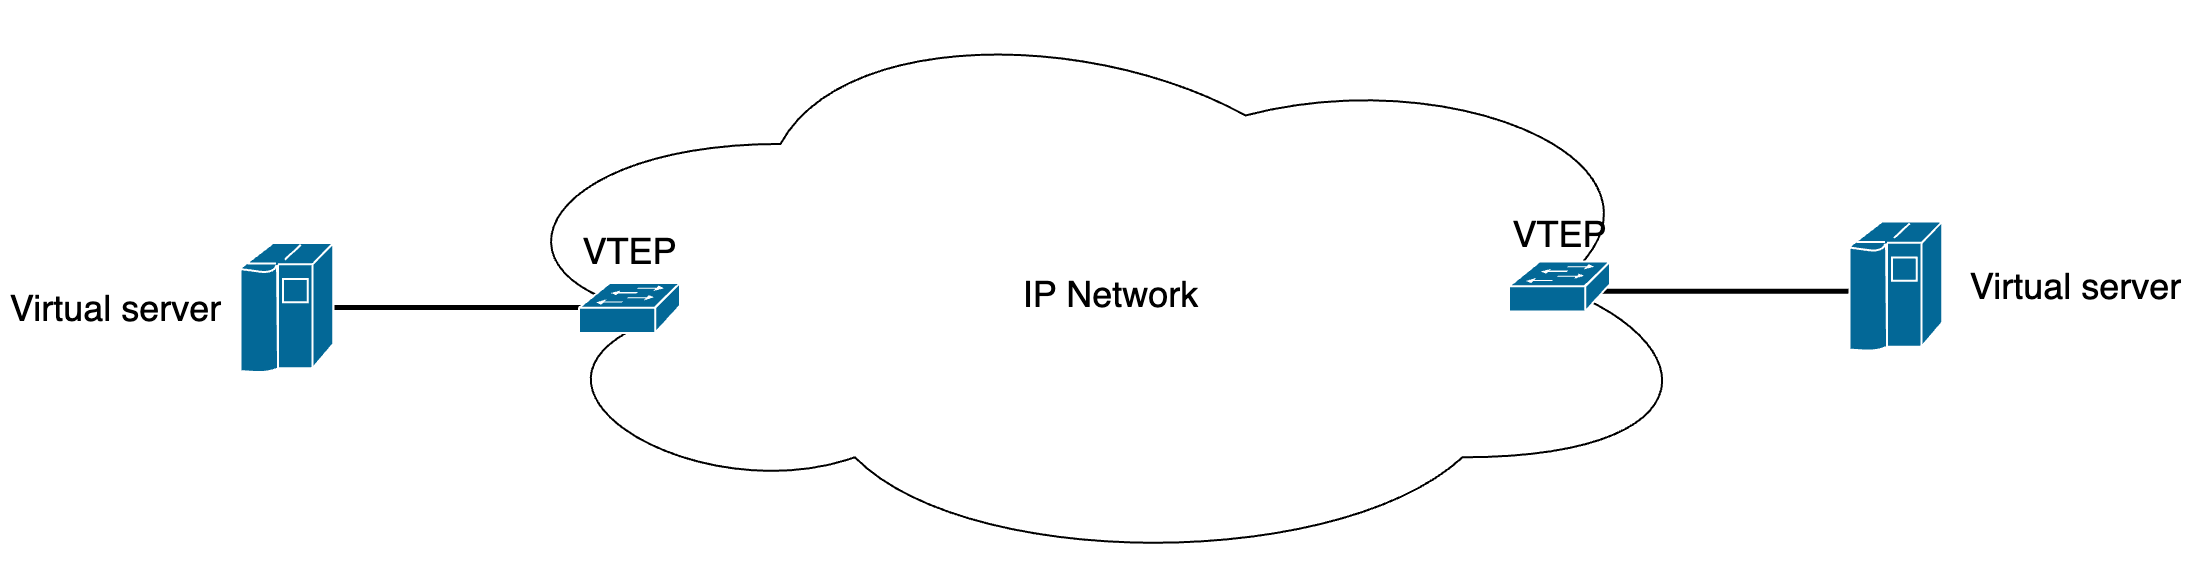
\includegraphics[width=\textwidth]{images/vtep.png}
  \end{figure}

  VXLAN (Virtual Extensible Local Area Network) --- это технология сетевой
  виртуализации, которая инкапсулирует пакеты данных, отправленные от
  виртуальных машин, в пакеты UDP.

  \vspace*{1em}

  VTEP (VXLAN tunnel endpoint) --- это конечные точки, которые инкапсулируют и
  декапсулируют пакеты VXLAN.
\end{frame}

\begin{frame}
  \frametitle{VXLAN}

  \begin{figure}[H]
    \centering
    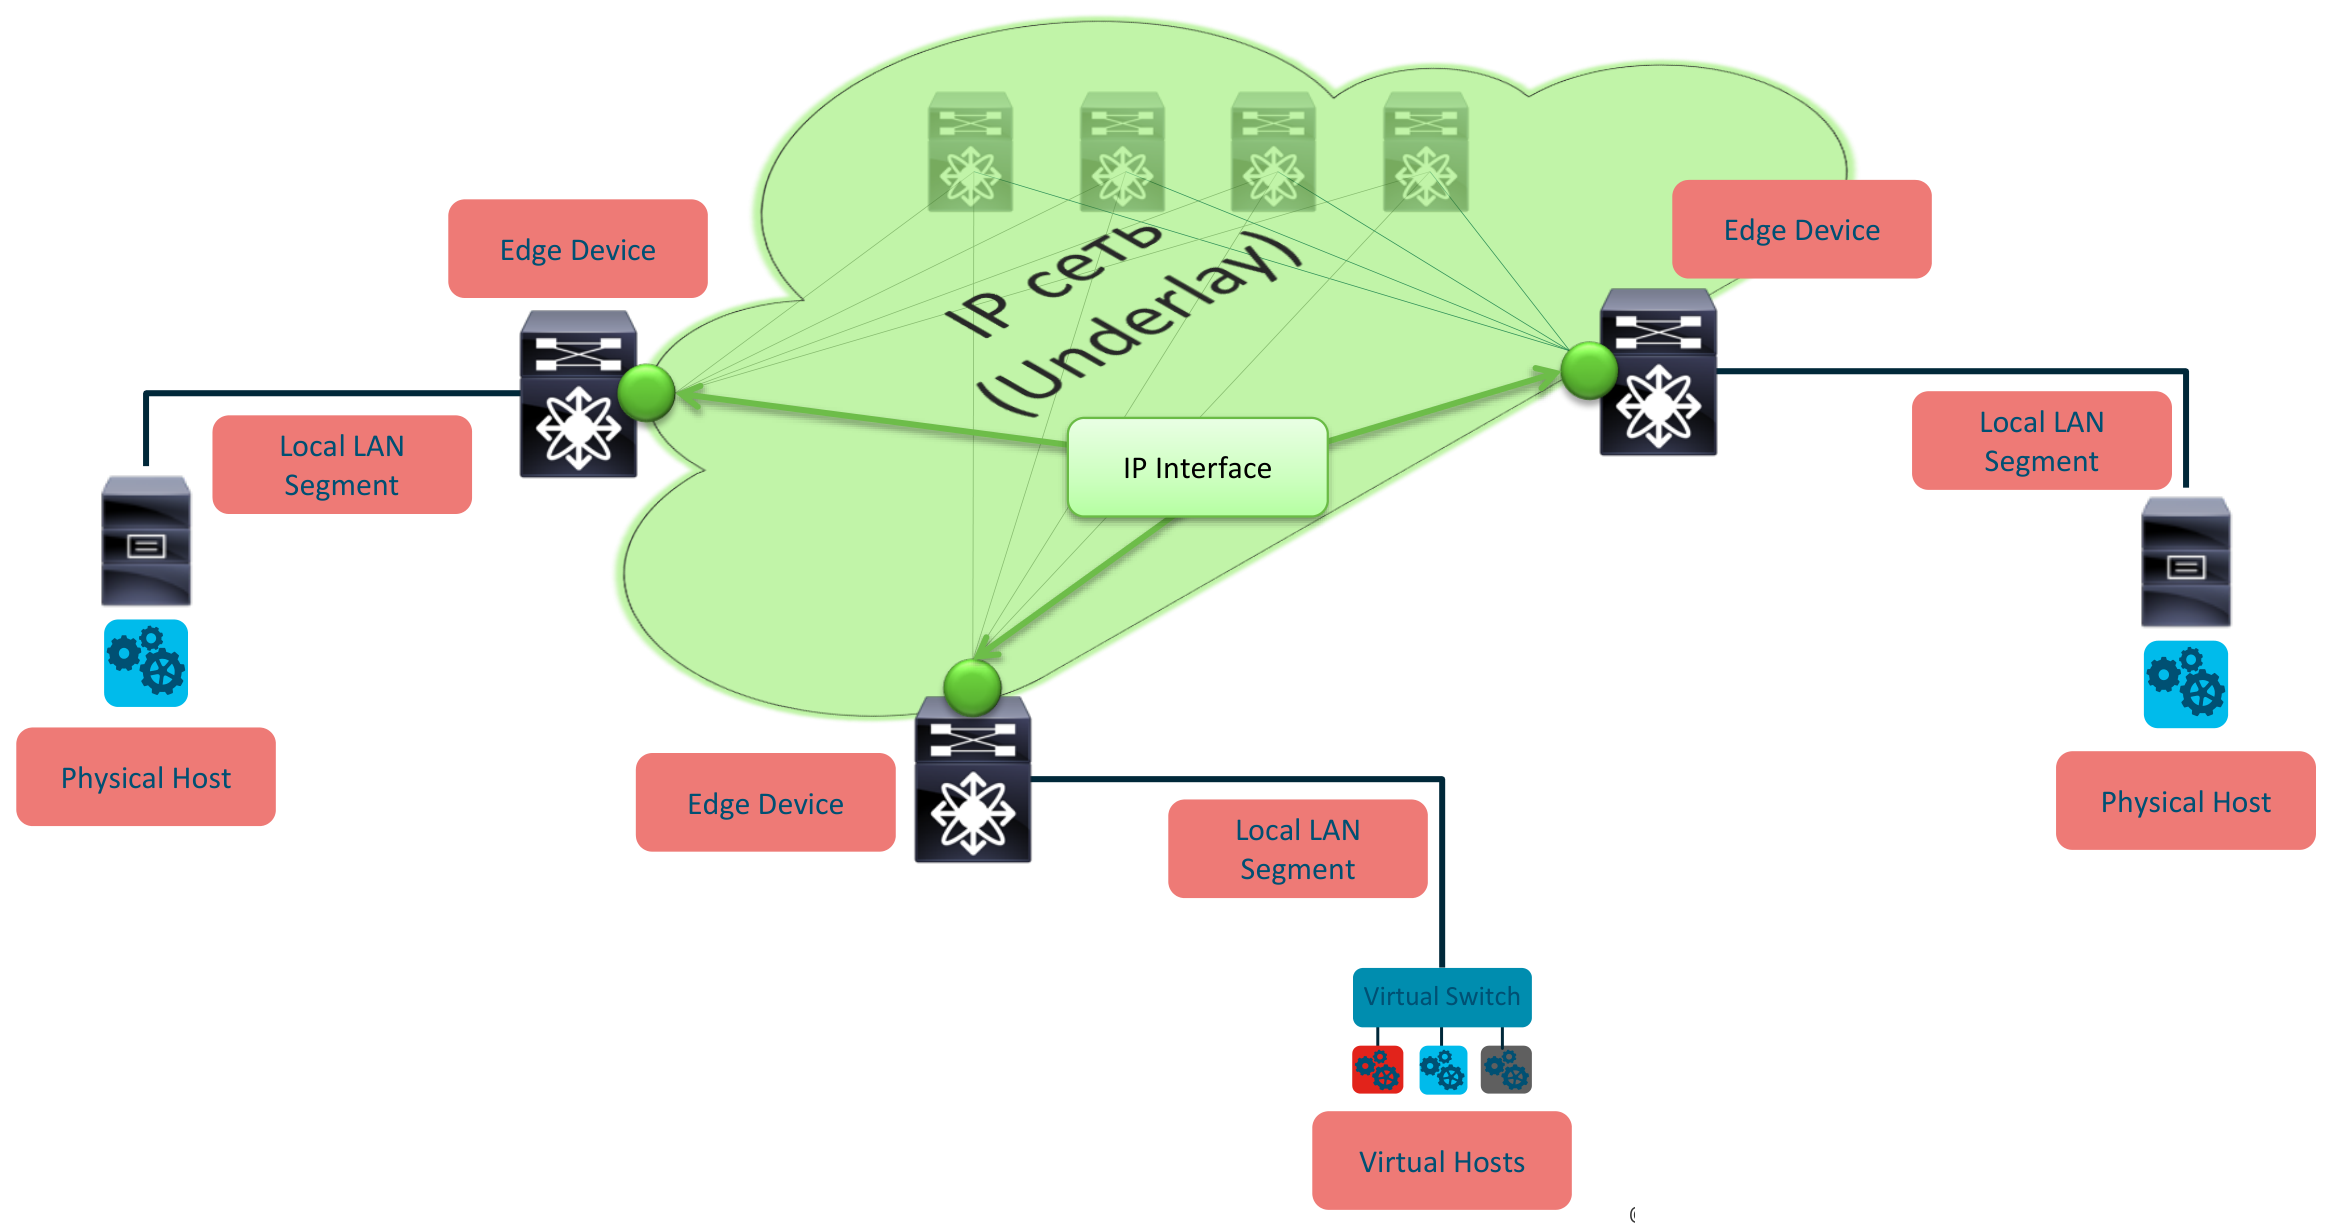
\includegraphics[width=\textwidth]{images/underlay.png}
  \end{figure}
\end{frame}

\begin{frame}
  \frametitle{VXLAN}

  \begin{figure}[H]
    \centering
    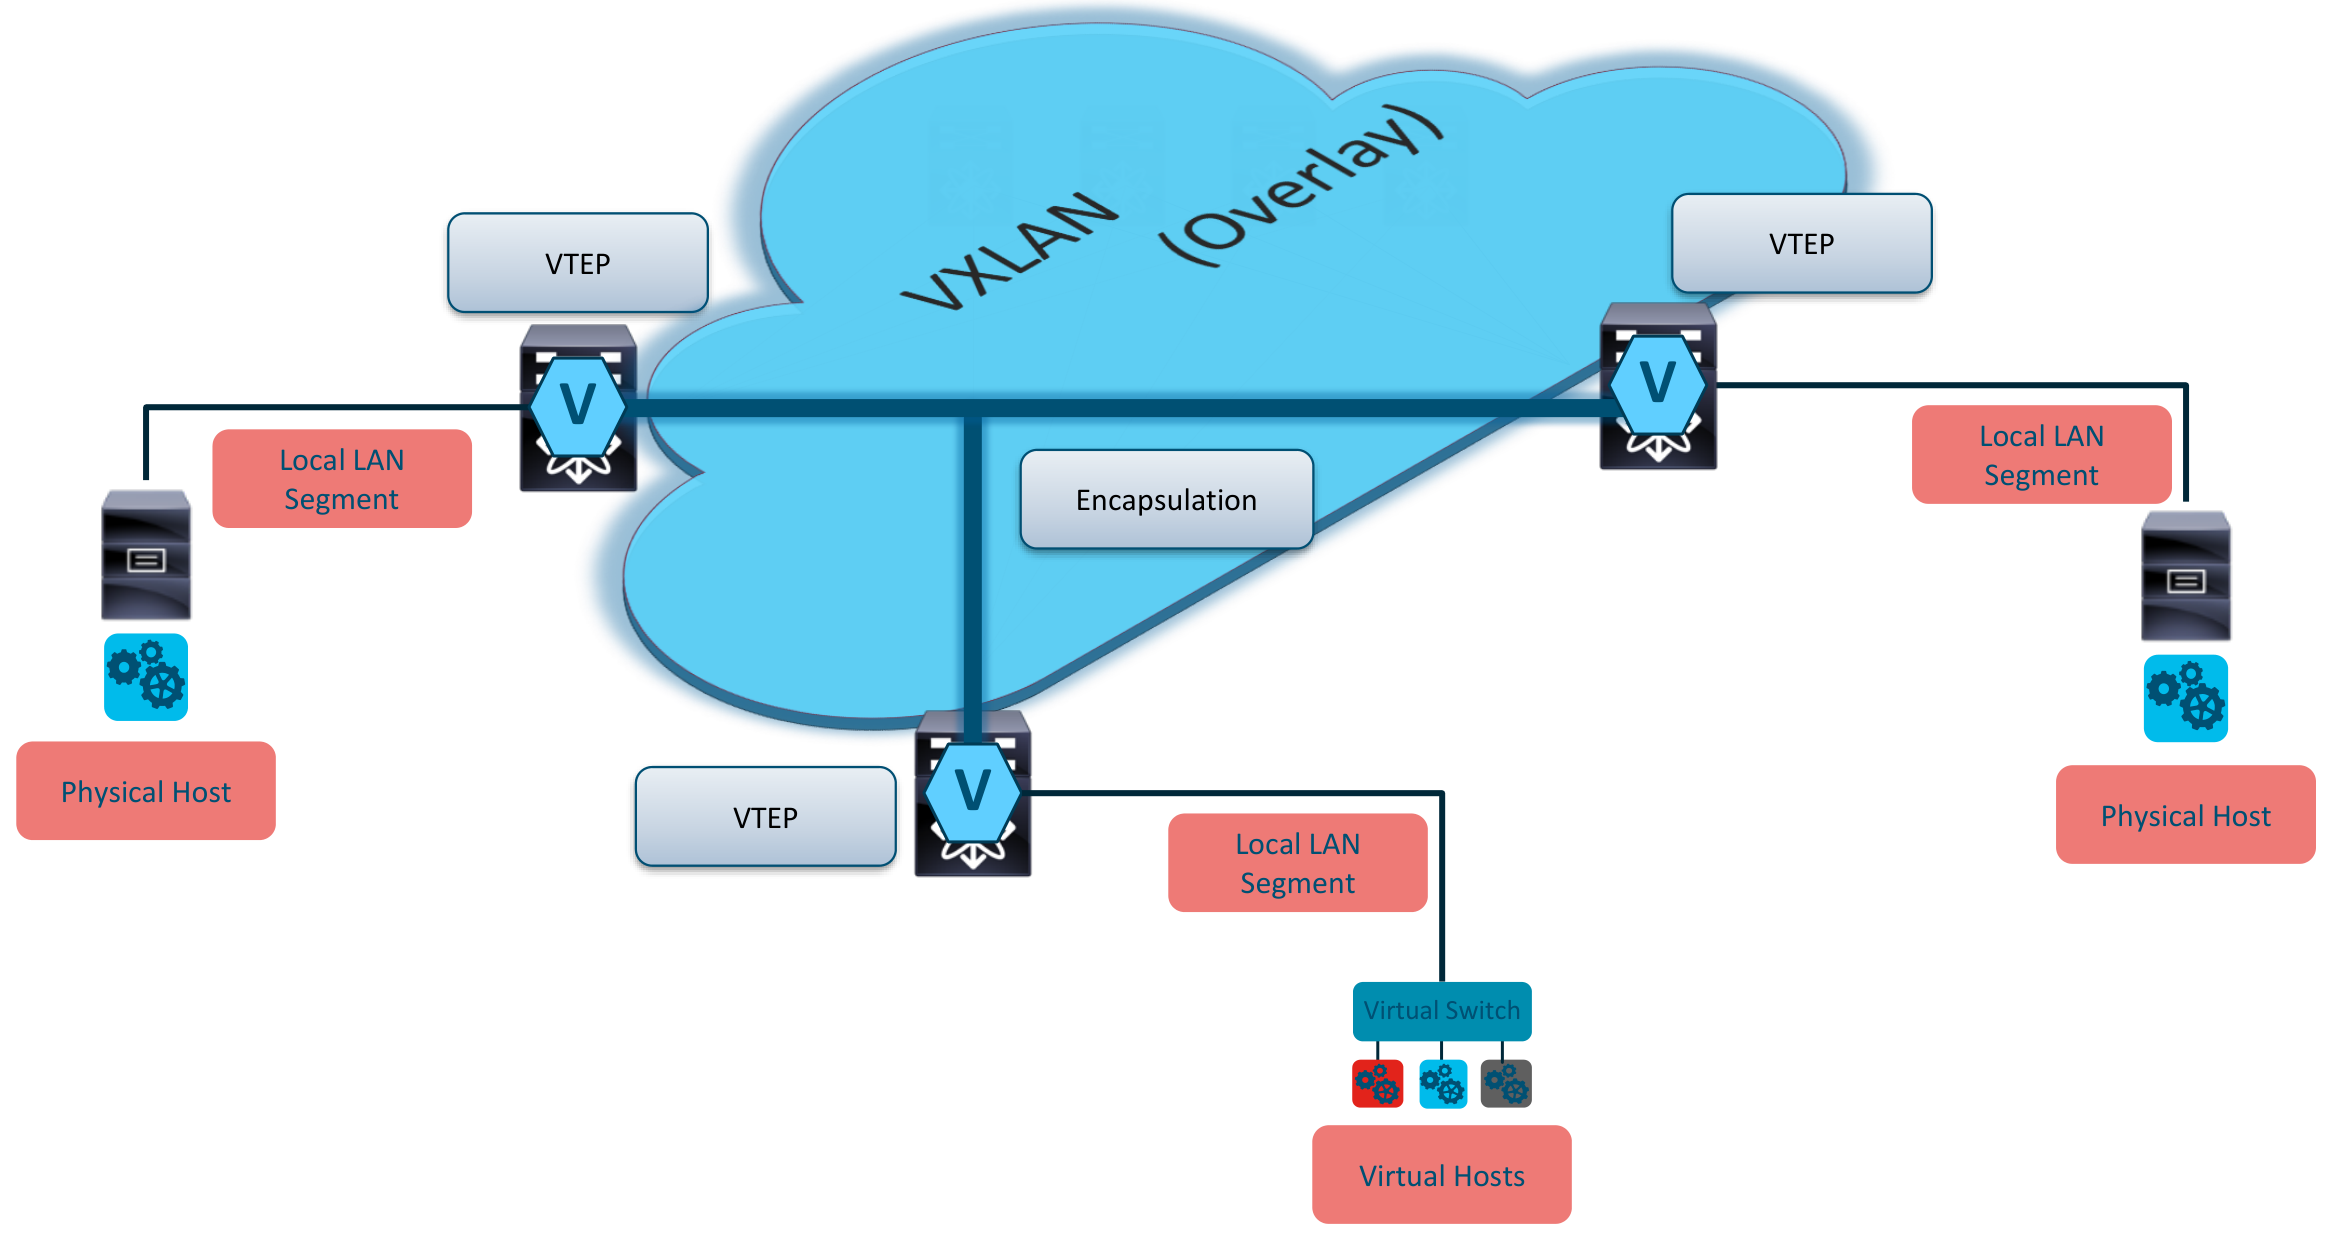
\includegraphics[width=\textwidth]{images/overlay.png}
  \end{figure}
\end{frame}

\begin{frame}
  \frametitle{Формат кадра VXLAN}

  VLAN кадр:
  \begin{center}
    \footnotesize
    \renewcommand*{\arraystretch}{3.0}
    \begin{tabularx}{\textwidth}{|c|C|c|}
      \hline
      \shortstack{Ethernet \\ 18 байт}          &
      \shortstack{Payload  \\ 1500 байт} &
      \shortstack{FSC      \\ 4 байта}         \\
      \hline
    \end{tabularx}
  \end{center}

  \vspace*{1em}

  VXLAN кадр:
  \begin{center}
    \footnotesize
    \renewcommand*{\arraystretch}{3.0}
    \begin{tabularx}{\textwidth}{|c|c|c|c|c|C|c|}
      \hline
      \shortstack{Outer Ethernet \\ 14 байт}          &
      \shortstack{Outer IP       \\ 20 байт}          &
      \shortstack{UDP            \\ 8 байт}          &
      \shortstack{VXLAN          \\ 8 байт}          &
      \shortstack{Inner Ethernet \\ 14 (18) байт}          &
      \shortstack{Payload        \\ 1500 байт} &
      \shortstack{FSC            \\ 4 байта}         \\
      \hline
    \end{tabularx}
  \end{center}
\end{frame}

\begin{frame}
  \frametitle{Формат кадра VXLAN}

  VXLAN кадр:
  \begin{center}
    \footnotesize
    \renewcommand*{\arraystretch}{3.0}
    \begin{tabularx}{\textwidth}{|c|c|c|c|c|C|c|}
      \hline
      \cellcolor{yellow!25}\shortstack{Outer Ethernet \\ 14 байт}          &
      \shortstack{IPv4                                \\ 20 байт}          &
      \shortstack{UDP                                 \\ 8 байт}          &
      \shortstack{VXLAN                               \\ 8 байт}          &
      \shortstack{Inner Ethernet                      \\ 14 (18) байт}          &
      \shortstack{Payload                             \\ 1500 байт} &
      \shortstack{FSC                                 \\ 4 байта}         \\
      \hline
    \end{tabularx}
  \end{center}

  \vspace*{1em}

  Формат Ethernet заголовка:
  \begin{center}
    \footnotesize
    \renewcommand*{\arraystretch}{3.0}
    \begin{tabularx}{\textwidth}{|C|C|C|}
      \hline
      \shortstack{Source MAC      \\ 6 байт}          &
      \shortstack{Destination MAC \\ 6 байт} &
      \shortstack{Type            \\ 2 байта}       \\
      \hline
    \end{tabularx}
  \end{center}

  \vspace*{1em}

  \begin{itemize}[label=,leftmargin=0pt]
    \item \textbf{Destination MAC}: MAC-адрес VTEP, на который будет отправлен
    пакет в соответствии с таблицей маршрутизации.
    \item \textbf{Source MAC}: MAC-адрес VTEP, на который виртуальная машина
    отправляет пакет.
    \item Все остальное заполняется также, как для обычного Ethernet.
  \end{itemize}
\end{frame}

\begin{frame}
  \frametitle{Формат кадра VXLAN}

  VXLAN кадр:
  \begin{center}
    \footnotesize
    \renewcommand*{\arraystretch}{3.0}
    \begin{tabularx}{\textwidth}{|c|c|c|c|c|C|c|}
      \hline
      \shortstack{Outer Ethernet            \\ 14 байт}          &
      \cellcolor{yellow!25}\shortstack{IPv4 \\ 20 байт}          &
      \shortstack{UDP                       \\ 8 байт}          &
      \shortstack{VXLAN                     \\ 8 байт}          &
      \shortstack{Inner Ethernet            \\ 14 (18) байт}          &
      \shortstack{Payload                   \\ 1500 байт} &
      \shortstack{FSC                       \\ 4 байта}         \\
      \hline
    \end{tabularx}
  \end{center}

  \vspace*{1em}

  Формат IPv4 заголовка:
  \begin{center}
    \footnotesize
    \renewcommand*{\arraystretch}{3.0}
    \begin{tabularx}{\textwidth}{|C|C|C|}
      \hline
      \shortstack{\ldots         \\ 12 байт} &
      \shortstack{Source IP      \\ 4 байта}          &
      \shortstack{Destination IP \\ 4 байта}          \\
      \hline
    \end{tabularx}
  \end{center}

  \vspace*{1em}

  \begin{itemize}[label=,leftmargin=0pt]
    \item \textbf{Source IP}: IP-адрес локального VTEP.
    \item \textbf{Destination IP}: IP-адрес удаленного VTEP.
    \item Все остальное заполняется также, как для обычного IPv4.
  \end{itemize}
\end{frame}

\begin{frame}
  \frametitle{Формат кадра VXLAN}

  VXLAN кадр:
  \begin{center}
    \footnotesize
    \renewcommand*{\arraystretch}{3.0}
    \begin{tabularx}{\textwidth}{|c|c|c|c|c|C|c|}
      \hline
      \shortstack{Outer Ethernet           \\ 14 байт}          &
      \shortstack{IPv4                     \\ 20 байт}          &
      \cellcolor{yellow!25}\shortstack{UDP \\ 8 байт}          &
      \shortstack{VXLAN                    \\ 8 байт}          &
      \shortstack{Inner Ethernet           \\ 14 (18) байт}          &
      \shortstack{Payload                  \\ 1500 байт} &
      \shortstack{FSC                      \\ 4 байта}         \\
      \hline
    \end{tabularx}
  \end{center}

  \vspace*{1em}

  Формат UDP заголовка:
  \begin{center}
    \footnotesize
    \renewcommand*{\arraystretch}{3.0}
    \begin{tabularx}{\textwidth}{|C|C|C|C|}
      \hline
      \shortstack{Source port      \\ 2 байта}          &
      \shortstack{Destination port \\ 2 байта}          &
      \shortstack{Length           \\ 2 байта}          &
      \shortstack{Checksum         \\ 2 байта}          \\
      \hline
    \end{tabularx}
  \end{center}

  \vspace*{1em}

  \begin{itemize}[label=,leftmargin=0pt]
    \item \textbf{Source Port}: вычисляется хешированием заголовков внутреннего
    кадра Ethernet.
    \item \textbf{Destination Port}: всегда равен 4789.
    \item Все остальное заполняется также, как для обычного UDP.
  \end{itemize}
\end{frame}

\begin{frame}
  \frametitle{Формат кадра VXLAN}

  VXLAN кадр:
  \begin{center}
    \footnotesize
    \renewcommand*{\arraystretch}{3.0}
    \begin{tabularx}{\textwidth}{|c|c|c|c|c|C|c|}
      \hline
      \shortstack{Outer Ethernet             \\ 14 байт}          &
      \shortstack{IPv4                       \\ 20 байт}          &
      \shortstack{UDP                        \\ 8 байт}          &
      \cellcolor{yellow!25}\shortstack{VXLAN \\ 8 байт}          &
      \shortstack{Inner Ethernet             \\ 14 (18) байт}          &
      \shortstack{Payload                    \\ 1500 байт} &
      \shortstack{FSC                        \\ 4 байта}         \\
      \hline
    \end{tabularx}
  \end{center}

  \vspace*{1em}

  Формат заголовка VXLAN:
  \begin{center}
    \footnotesize
    \renewcommand*{\arraystretch}{3.0}
    \begin{tabularx}{\textwidth}{|C|C|C|C|}
      \hline
      \shortstack{VXLAN Flags \\ 1 байт}          &
      \shortstack{Reserved    \\ 3 байта}          &
      \shortstack{VNI         \\ 3 байта}          &
      \shortstack{Reserved    \\ 1 байт}          \\
      \hline
    \end{tabularx}
  \end{center}

  \vspace*{1em}

  \begin{itemize}[label=,leftmargin=0pt]
    \item \textbf{VXLAN Flags}: пятый бит должен быть равен 1. Этот бит
    сигнализирует о том, что заголовок содержит корректный VNI. Остальные семь бит
    зарезервированы и равны 0.
    \item \textbf{VNI}: идентификатор виртуальной сети.
    \item \textbf{Reversed}: зарезервировано, все биты должны быть равны 0.
  \end{itemize}
\end{frame}

\begin{frame}
  \frametitle{Отличия VXLAN от VLAN}

  VLAN кадр:
  \begin{center}
    \footnotesize
    \renewcommand*{\arraystretch}{3.0}
    \begin{tabularx}{\textwidth}{|c|C|c|}
      \hline
      \shortstack{Ethernet \\ 18 байт}          &
      \shortstack{Payload  \\ 1500 байт} &
      \shortstack{FSC      \\ 4 байта}         \\
      \hline
    \end{tabularx}
  \end{center}

  \vspace*{1em}

  VXLAN кадр:
  \begin{center}
    \footnotesize
    \renewcommand*{\arraystretch}{3.0}
    \begin{tabularx}{\textwidth}{|c|c|c|c|c|C|c|}
      \hline
      \shortstack{Outer Ethernet \\ 14 байт}          &
      \shortstack{Outer IP       \\ 20 байт}          &
      \shortstack{UDP            \\ 8 байт}          &
      \shortstack{VXLAN          \\ 8 байт}          &
      \shortstack{Inner Ethernet \\ 14 (18) байт}          &
      \shortstack{Payload        \\ 1500 байт} &
      \shortstack{FSC            \\ 4 байта}         \\
      \hline
    \end{tabularx}
  \end{center}

  \vspace*{1em}

  \begin{itemize}
    \item максимальное количество виртуальных сетей, поддерживаемых VXLAN,
    составляет более 16 миллионов;
    \item для конфигурации VXLAN реконфигурация физического сетевого
    оборудования не требуется.
  \end{itemize}
\end{frame}

\begin{frame}
  \frametitle{Итого имеем}

  \begin{figure}[H]
    \centering
    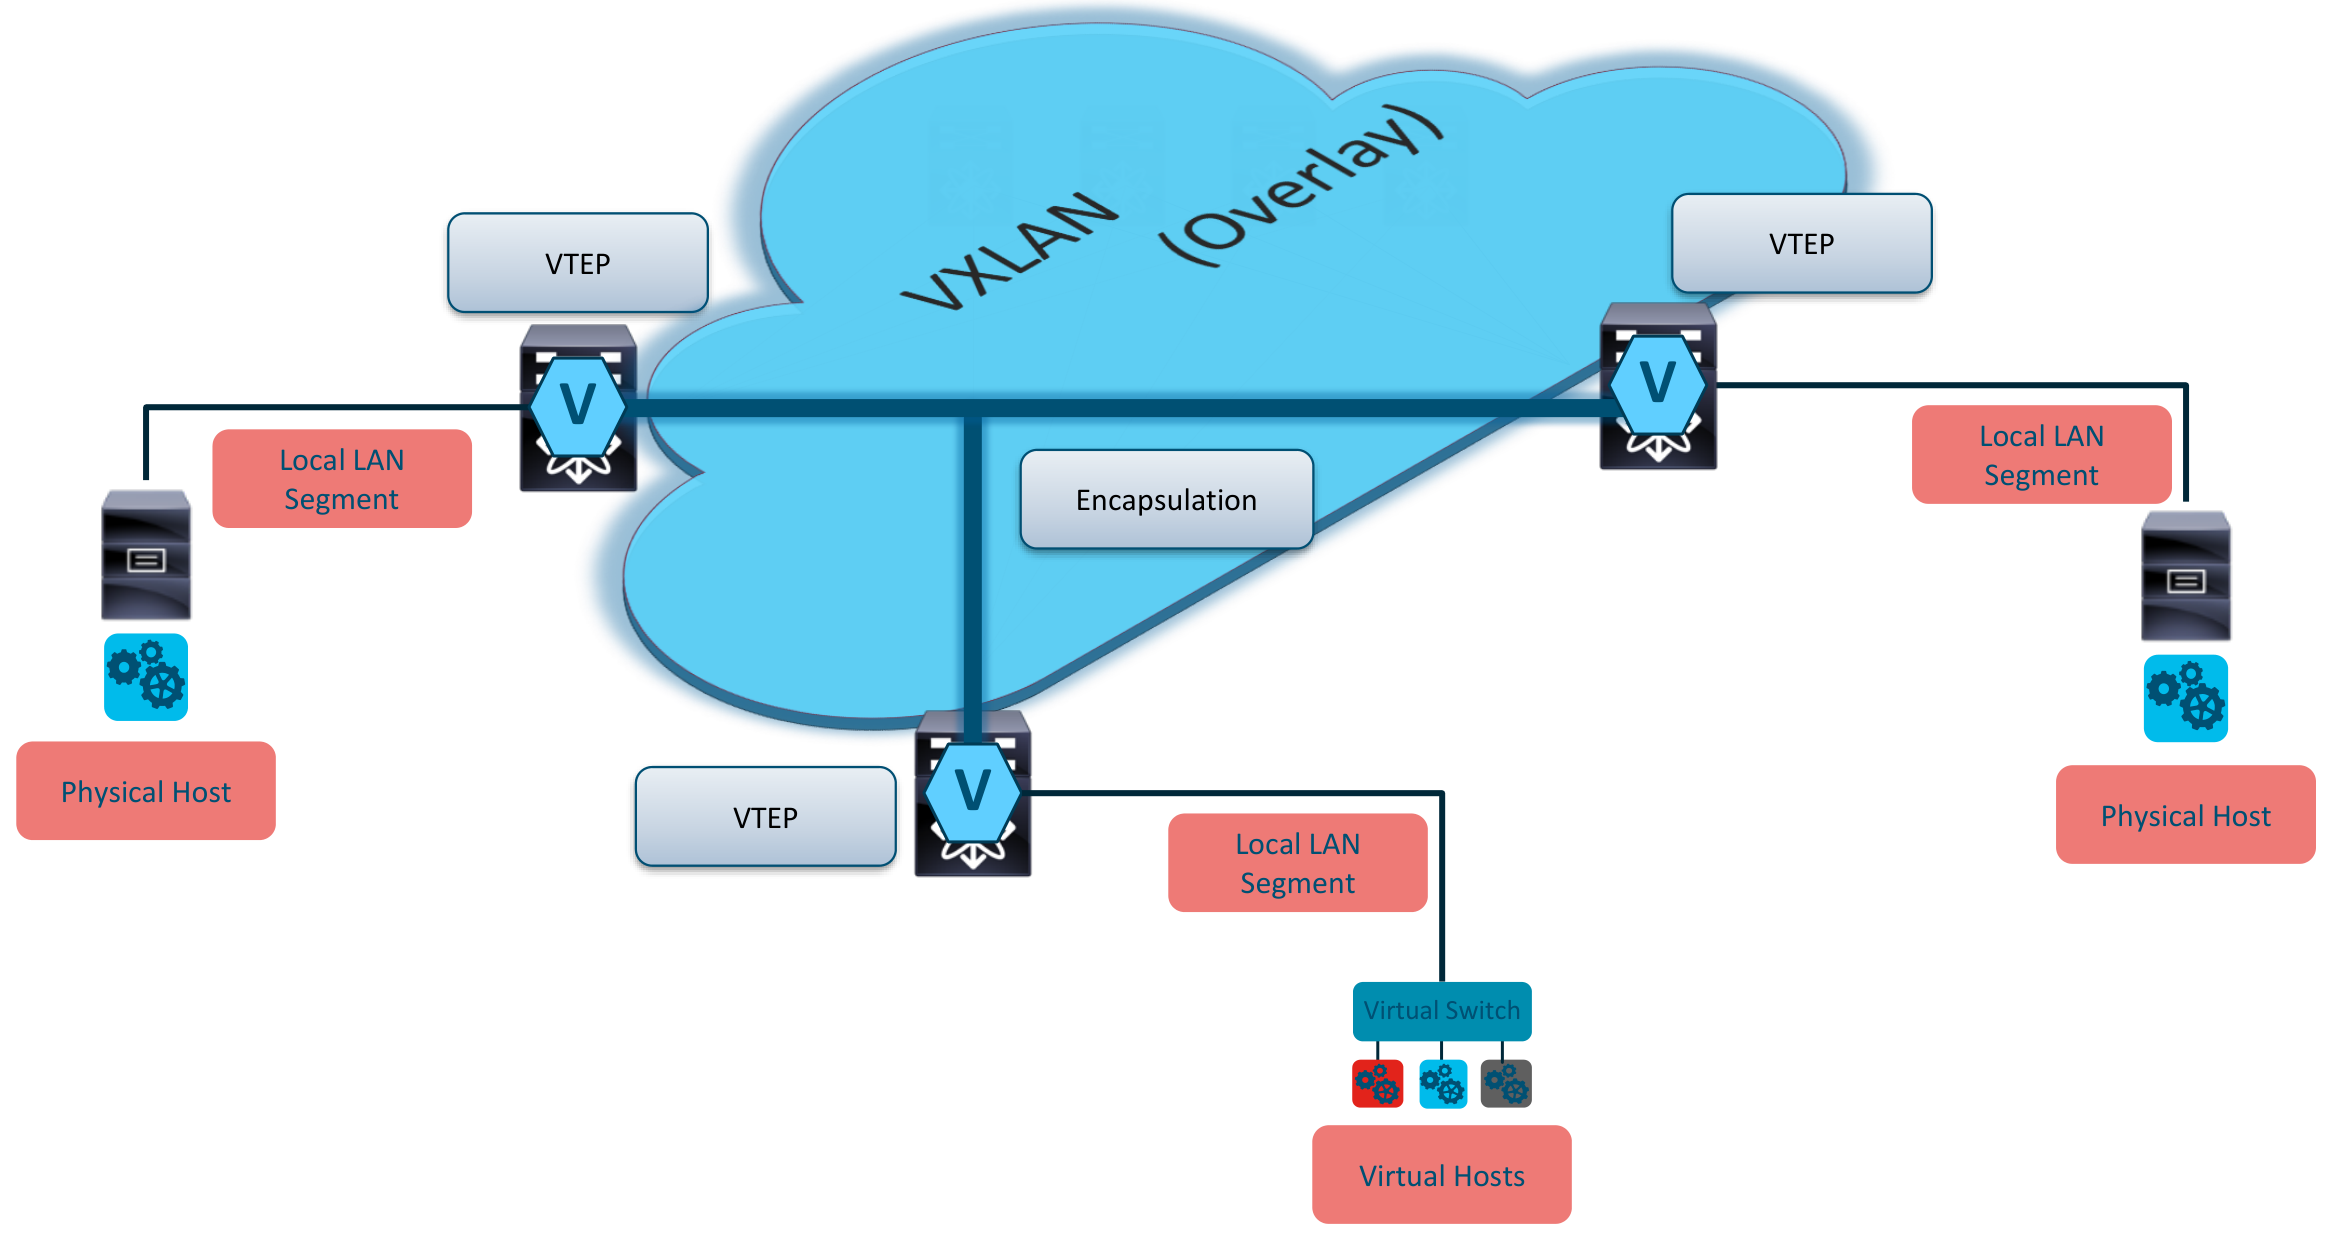
\includegraphics[width=0.7\textwidth]{images/overlay.png}
  \end{figure}

  VXLAN --- это технология сетевой виртуализации, которая инкапсулирует пакеты
  данных, отправленные от виртуальных машин, в пакеты UDP. VXLAN позволяет
  большому количеству арендаторов предоставлять услуги доступа к виртуальной сети.
\end{frame}

\begin{frame}
  \frametitle{Спасибо за внимание}

  \begin{figure}[H]
    \centering
    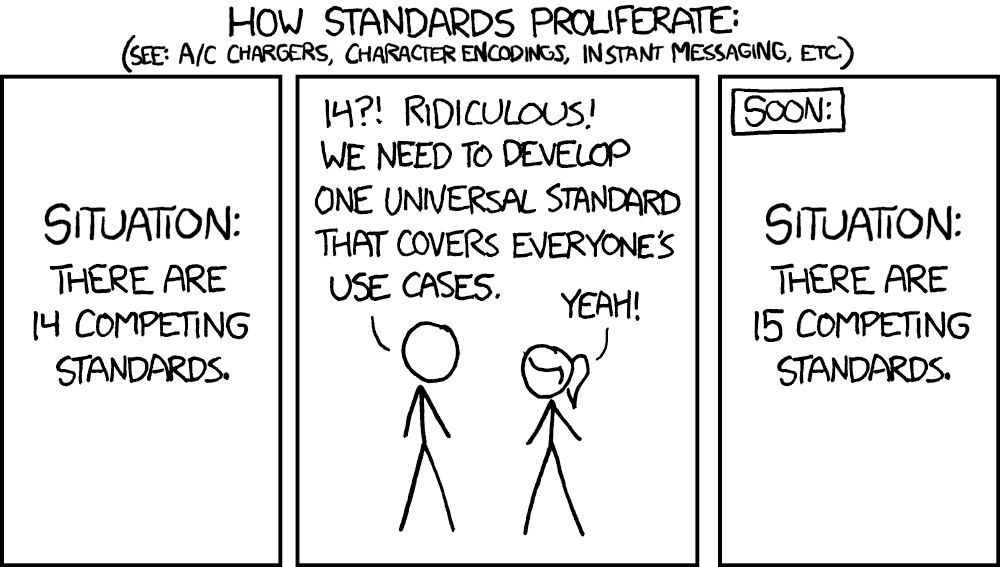
\includegraphics[width=0.7\textwidth]{images/standards_2x.png}
    \caption{Мемчик напоследок}
  \end{figure}
\end{frame}

\end{document}
